\documentclass[10pt,twocolumn,letterpaper]{article}

\usepackage{cvpr}
\usepackage{times}
\usepackage{epsfig}
\usepackage{graphicx}
\usepackage{amsmath}
\usepackage{amssymb}

% Include other packages here, before hyperref.

% If you comment hyperref and then uncomment it, you should delete
% egpaper.aux before re-running latex.  (Or just hit 'q' on the first latex
% run, let it finish, and you should be clear).
\usepackage[breaklinks=true,bookmarks=false]{hyperref}

\cvprfinalcopy % *** Uncomment this line for the final submission

\def\cvprPaperID{****} % *** Enter the CVPR Paper ID here
\def\httilde{\mbox{\tt\raisebox{-.5ex}{\symbol{126}}}}

% Pages are numbered in submission mode, and unnumbered in camera-ready
%\ifcvprfinal\pagestyle{empty}\fi
\setcounter{page}{1}
\begin{document}

%%%%%%%%% TITLE
\title{Project: Car detection on KITTI dataset}

\author{Muhammad Haris Ibrahim\\
{\tt\small muhammad.ibrahim@student.uni-luebeck.de}
% For a paper whose authors are all at the same institution,
% omit the following lines up until the closing ``}''.
% Additional authors and addresses can be added with ``\and'',
% just like the second author.
% To save space, use either the email address or home page, not both
}

\maketitle
%\thispagestyle{empty}

%%%%%%%%% ABSTRACT
\begin{abstract}
  Detecting cars on the road is a critical task for autonomous driving. This must be done with high precision, high recall and in real-time. 
  In this paper, we develop a 2D car detector by fine tuning the YOLO-v3 object detector to detect cars on a scaled down version of KITTI dataset. 
  We achieved 51 percent mean Average Precision after finetuning YOLO-v3 model previously trained on MS COCO dataset. 
  Improvements to the training process are required to achieve better results.
\end{abstract}

%%%%%%%%% BODY TEXT
\section{Introduction}
Object detection is a critical task for autonomous driving. An autonomous vehicle must be able to detect and keep track of objects of interest in its environment. The classification of objects is not enough, their position and orientation in the environment must also be predicted. 
Another challenge is that these detections must be performed at high precision and recall but also in real-time on edge devices. The objects of interest can be lane line markings, traffic signs, vehicles, pedestrians and more. 

In this project, we focus only on detecting cars. Car detection is specially important in autonomous driving to avoid collisions and plan safe trajectories even at low levels of autonomy.

There are many deep learning based approaches for object detection. We adapt YOLO-v3 \cite{redmon2018yolov3}, a general purpose 2D object detector based on a Convolutional Neural Network (CNN) architecture. For training and evaluating our car detector, we will use a simplified version of KITTI dataset containing cars with 2D bounding box labels \cite{KITTI}.

YOLO-v3 is an improved version of YOLO \cite{redmon2016yolov1} which achieves 
higher mean Average Precision (mAP) on 2D object detection datasets like MS-COCO \cite{mscoco} while still being real-time. YOLO-v3 is a end to end CNN and performs predictions in only 1 pass.  

\begin{figure}[t]
	\begin{center}
		%\fbox{\rule{0pt}{2in} \rule{0.9\linewidth}{0pt}}
		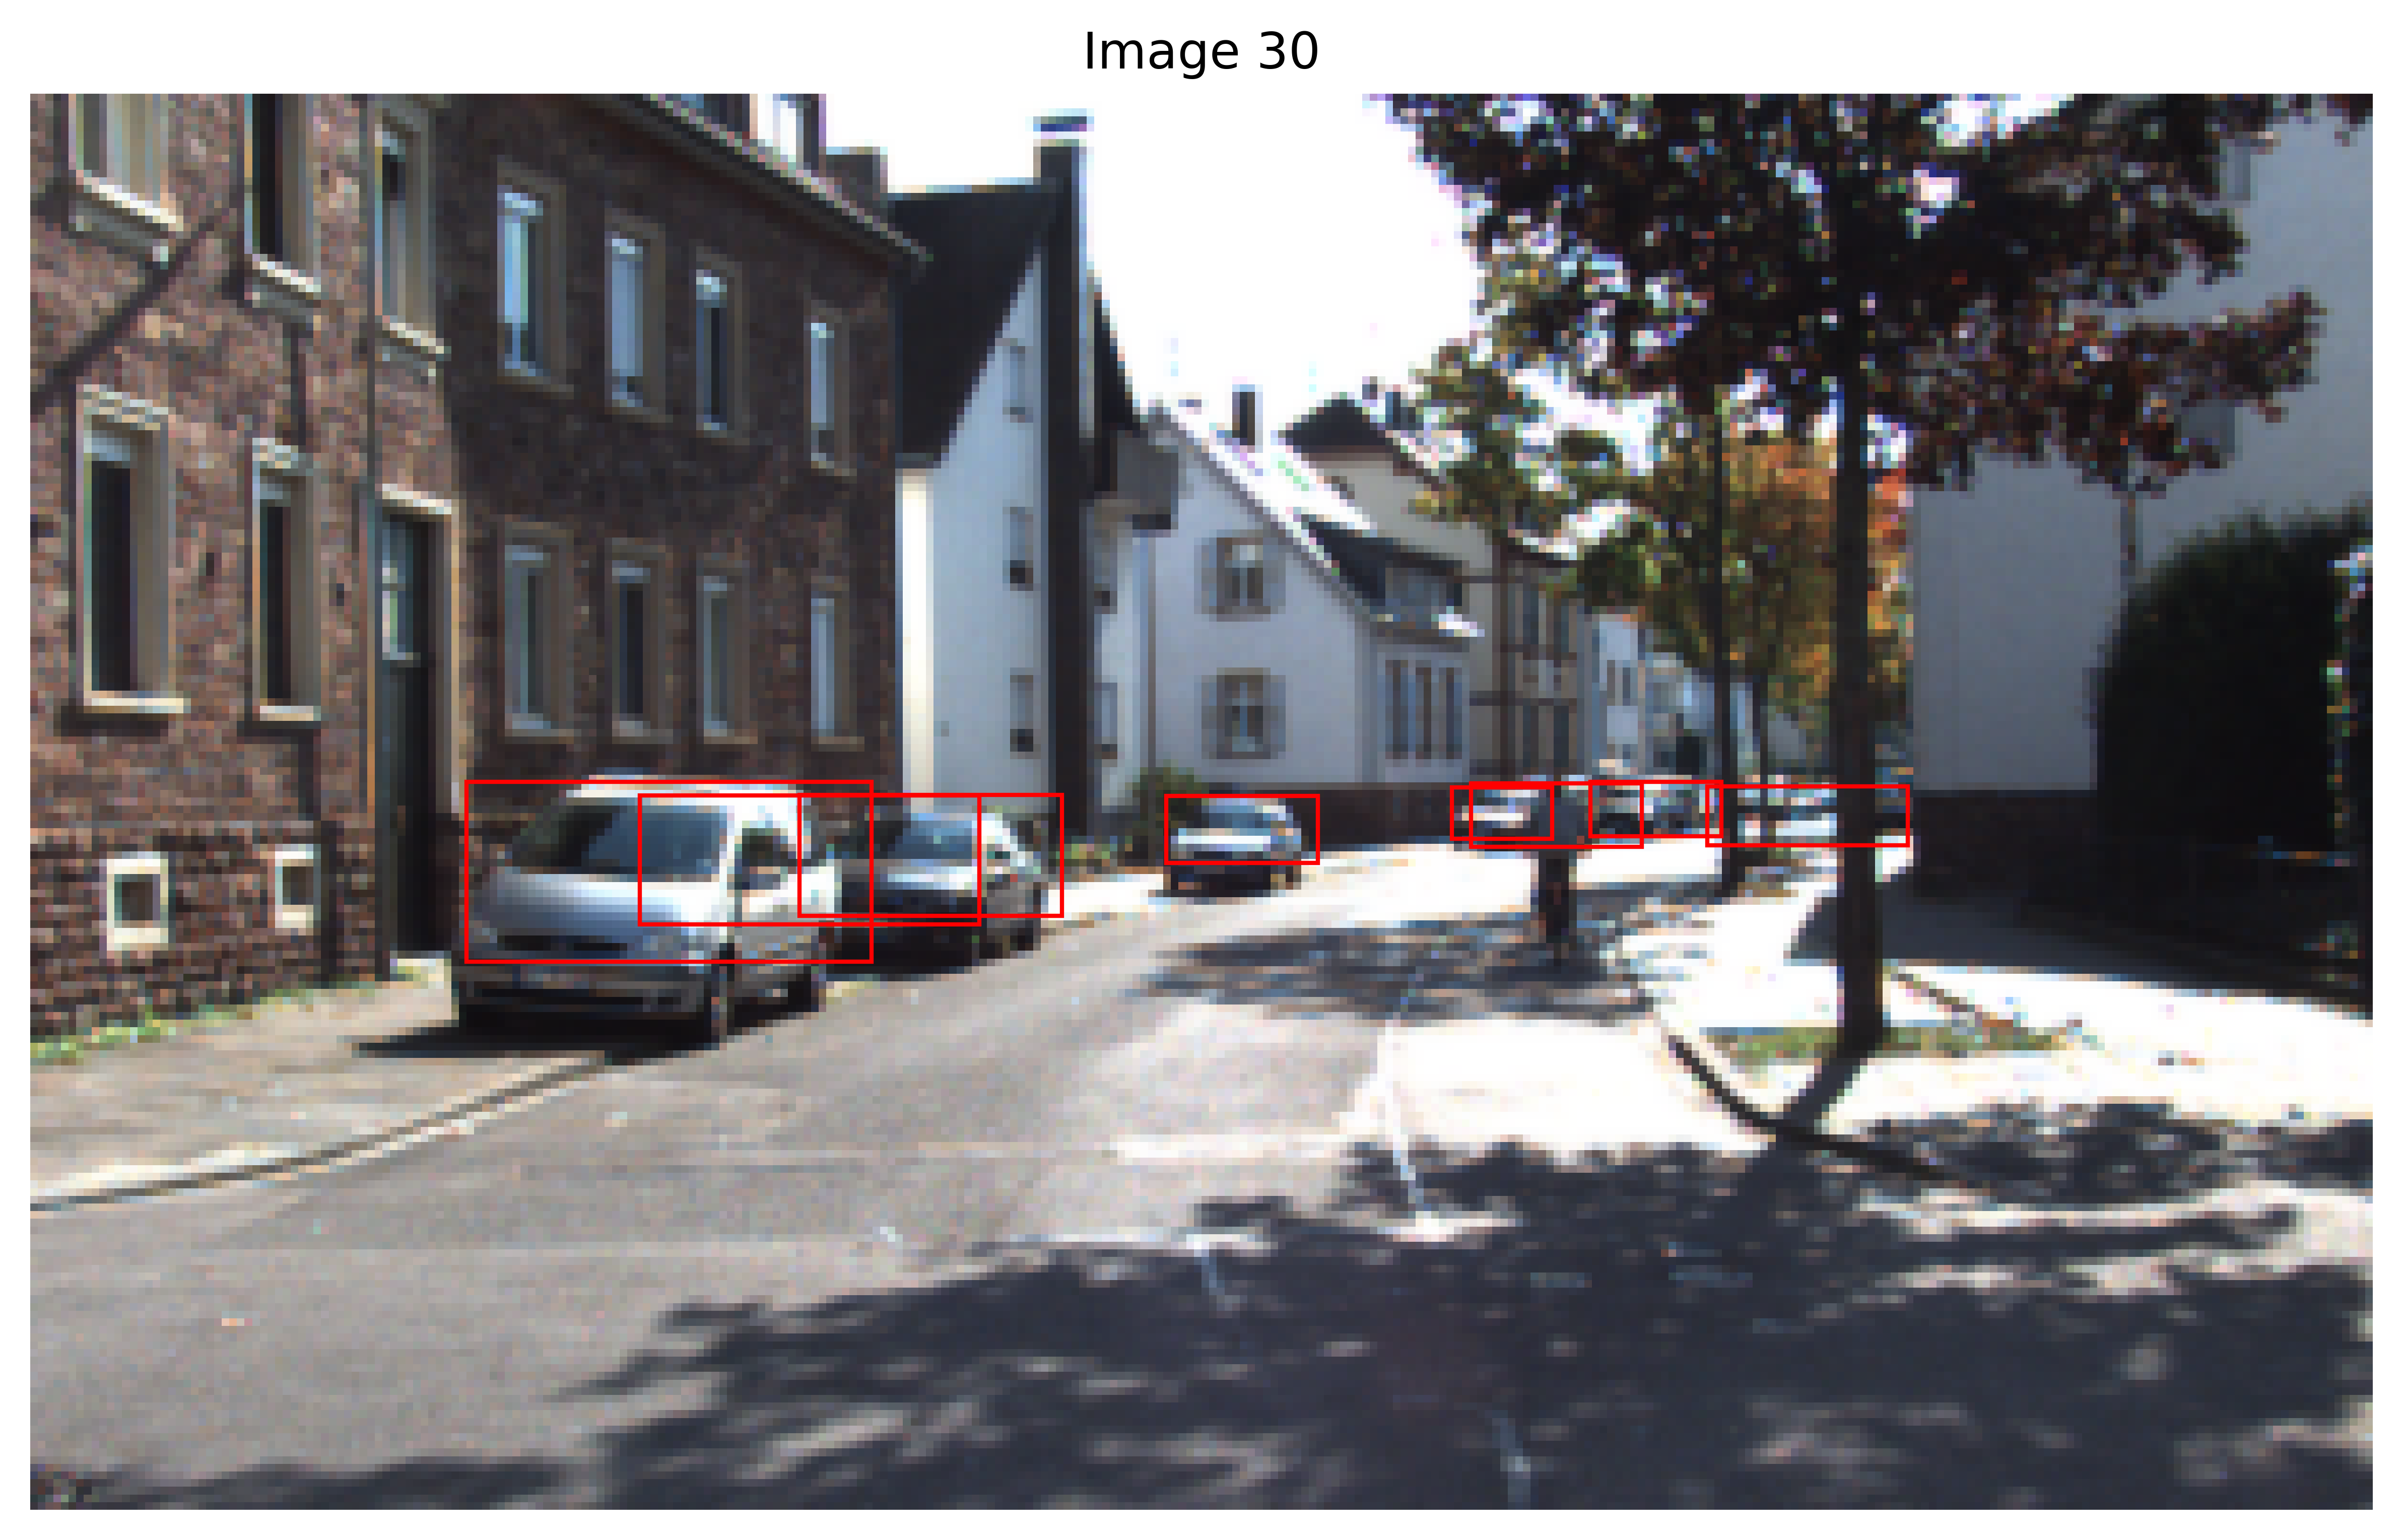
\includegraphics[width=1.0\linewidth]{figure30.png}
	\end{center}
	\caption{Detections of the model developed in this project on a sample image from the test set.}
	\label{fig:pred_example_plot}
\end{figure}

Transfer learning is then used to finetune it for car detection on our version of KITTI dataset. We obtained 51 percent mean Average Precision (mAP) on a validation set.
%-------------------------------------------------------------------------
\section{Related Work}
Since the success of Convolutional Neural Network (CNN) based approaches like Alexnet \cite{Alexnet} on image classification tasks, many similar approaches have been designed for object detection. Region Proposal CNNs (RCNN) \cite{ren2015faster} and its various variants use handcrafted algorithms to generate proposals for regions of interest. These proposals are then passed to a CNN which produces class and confidence predictions. The predictions are then fed back into the region proposal algorithm. This means that multiple passes are required to perform good predictions. This makes these networks slow at inference time. These multi-stage detectors are, therefore, not realtime. 

YOLO architecture and Single Shot Detector \cite{SSD_v1} solved this problem by performing the object detection in only one evaluation of the network. These are end to end CNNs. Out of these two, YOLO is the fastest. 

YOLO architecture frames the object detection problem as a regression problem. It divides the image into a SxS grid, where S is the grid size. For each of these grid cells, there are three bounding box predictors in the output layer. A bounding box prediction consists of 4 coordinates of the bounding box. Each grid cell also includes a class prediction. 

YOLO-v3 also divides the images into SxS cell, but it produces class probabilities for each bounding box not just for each grid cell. Predictions are also made at three different scales. Prediction of the bounding box coordinates are also as offsets of bounding box priors (anchor boxes). These anchor boxes are based on shapes of bounding boxes common for the problem. The network outputs a large number of predictions. Bounding box and class predictions are made at 3 scales, SxS grid cells per scale, and 3 per grid cells. Non Maximum Suppression (NMS) is applied to keep only the best predictions. YOLO-v3 has already been applied to many object detection problems like face detection \cite{face_detection_yolo}, predestrian detection \cite{pedestrian_detection} and much more.

A brief comparison of the performance of many object detection frameworks in shown in Figure \ref {fig:detector_comparison}.

There are more recent and improved versions of YOLO such as \cite{yolov7} that are not developed by the original authors. Recent works like Detection Transformer \cite{DETR} use a CNN backbone with a transformer encoder and decode blocks. These approaches achieve higher mAP precision. They also remove the need for anchor boxes and NMS. Because of the limits of the dataset, limited time and GPU compute, we use the YOLOv3 architecture and not the newer ones.

\begin{figure}[t]
	\begin{center}
		%\fbox{\rule{0pt}{2in} \rule{0.9\linewidth}{0pt}}
		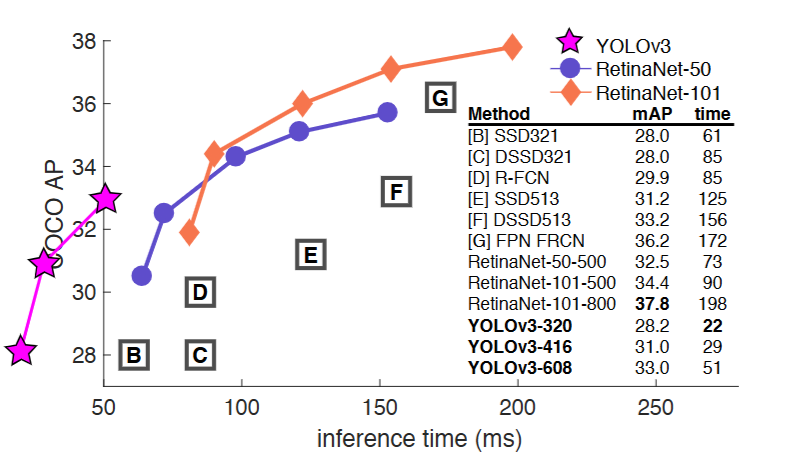
\includegraphics[width=1.0\linewidth]{object_detector_comparisons.png}
	\end{center}
	\caption{speed (ms) vs accuracy (AP) on MS. COCO test set. YOLOv3 outperforms many multistage and single stage object detectors in AP while being faster than all of them. This image is adapted from \cite{redmon2018yolov3} which is itself a version of image from \cite{retinaNet}}
	\label{fig:detector_comparison}
\end{figure}

\section{Method}
In this section, we provide a summary of the YOLO-v3 architecture. You should skip to the evaluation section to learn about the specific adaptions done by us.
\subsection{Bounding Boxes}
YOLO-v3 like many other object detectors does not predict the absolute coordinates of the bounding box. The bounding box centre coordinates are predicted as offsets to position of the top left corner of the grid cell. The width and height of the box are predicted as offset of the width and height of anchor boxes. These anchor boxes are pre-defined based on the likely shapes of anchor boxes for the problem at hand. The bounding box offsets are $t_x$, $t_y$, $t_w$, $t_h$. If the position of the top left of grid cell relative to the top left of the image is given by $(c_x, c_y)$ and the bounding box has width and height $p_w$, $p_h$, then the bounding box coordinates are calculated by: 
\begin{align*}
b_x &= \sigma(t_x) + c_x \\
b_y &= \sigma(t_y)  + c_y\\
b_w &= p_w e^{t_w}\\
b_h &= p_h e^{t_h}\\
\end{align*}
The ground truth values will be the left side of the above eqautions. We rearrange the equations to find the ground truth offsets.

The authors used clustering analysis to find the anchor box dimensions which have the most overlap with ground truth boxes on MS COCO dataset. We did not do such analysis on our dataset and used the anchor box dimension from the orignal source code.

There are 09 anchors boxes---03 at each scale. Each grid cells within a scale, predicts three bounding boxes as offsets of these anchors boxes. The anchor boxes are in sets of three where the size of boxes in each set is according to the prediction scale.

\subsection{Objectness Score}
Along with 04 coordinates of the bounding box, the network also predicts a objectness score for the bounding box. At test time, this is the confidence of the model in predicting that an object exists in the box and how well the box fits the object. At training time, this score should be the interesection over union between the predicted box and the ground truth box. The loss function forces this behaviour.

\subsection{Class Predictions}
The network predicts a class probability for each bounding box. At training time, we use Cross entropy loss for classification prediction of the box. This is probability that there exists an object of class i given that there is an object in the box, $\Pr(\textrm{Class}_i | \textrm{Object})$. We can multiply this by objectness score to get the classification confidence.

\subsection{Features extraction backbone}
The backbone of the network is a 53 layer CNN named as Darknet 53. The overall summary of the layers is shown in Table \ref{network_architecture}. 

\begin{table}[h] 
\begin{center}
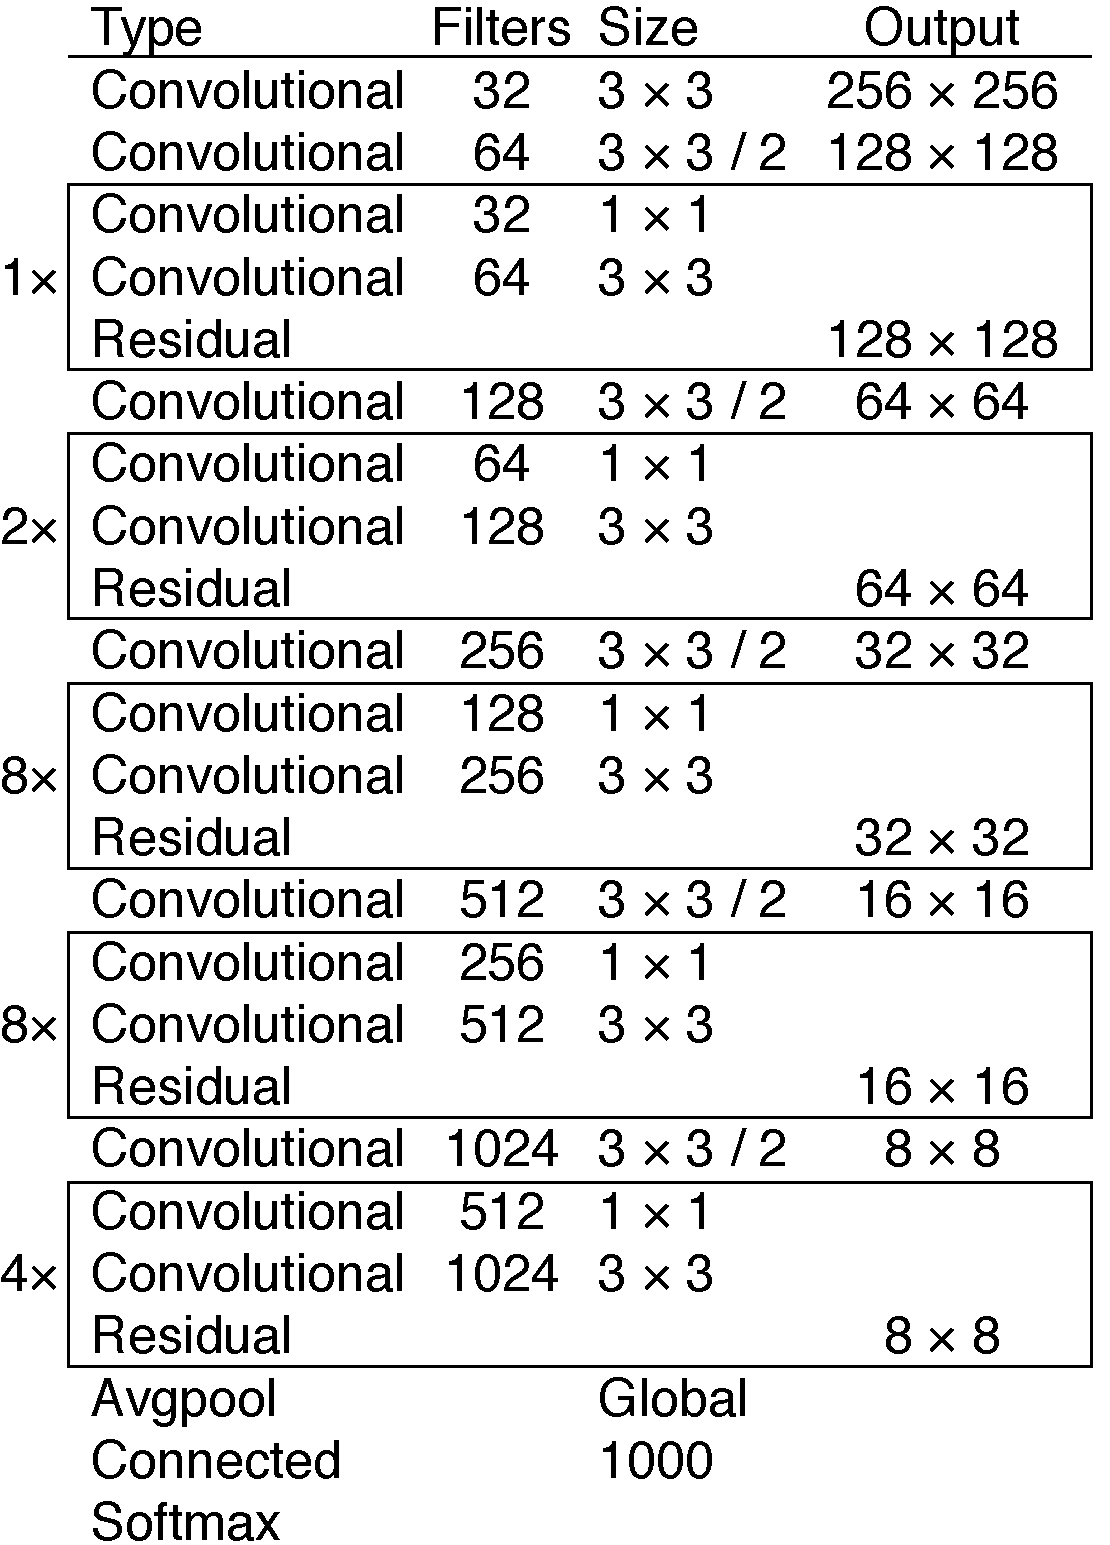
\includegraphics[width=.8\linewidth]{arch2.pdf}
\end{center}
\caption{\small \textbf{Darknet-53.}}
\label{network_architecture}
\end{table}

The authors did not explain any further details about the backbone. After spending sometime with the source code, our understanding is that each CNN block in the Table consists of a CNN layer, followed by leaky ReLU activation layer, and lastly a Batch Normalization layer. The filter sizes are mentioned in the Table. The 1x, 2x and such labels in the Table show the number of repeats. So, 2x means that such a block is repeated 2 times. It should be noted that the architecture includes skip connections like Resnets \cite{Resnets}. The authors trained this backbone for image classification on ImageNet dataset \cite{imagenet_dataset}. Further details about the training process were not provided. We assume a strategy similar to the YOLO-v1 was used.

\subsection{Three Scale Predictions}
The extracted features of the backbone are then passed to the detection heads at three different scales. This is inspired by Feature Pyramid Networks \cite{Feature_pyramids}. The size of the outputs are decided by dividing the image into SxS grid. There are three different grid sizes for three different scales. The idea is to use a larger grid size to help detect large object, then a medium size grid and then finally a smaller grid size. At each scale, the network has SxS predictors. Each grid cell has three predictors. Each predictor then predicts 4 bounding box coordinates (as offsets to three anchors), 1 objectness score and C class probabilities for C classes. So the total predictions at each scale are $S\times S\times [3*(4+1+C)]$. 
After the output of the feature extract backbone, several convolutional layers are added. The overall structure can be seen in Figure \ref{fig:detection_head}

\begin{figure*}[t]
	\begin{center}
		%\fbox{\rule{0pt}{2in} \rule{0.9\linewidth}{0pt}}
		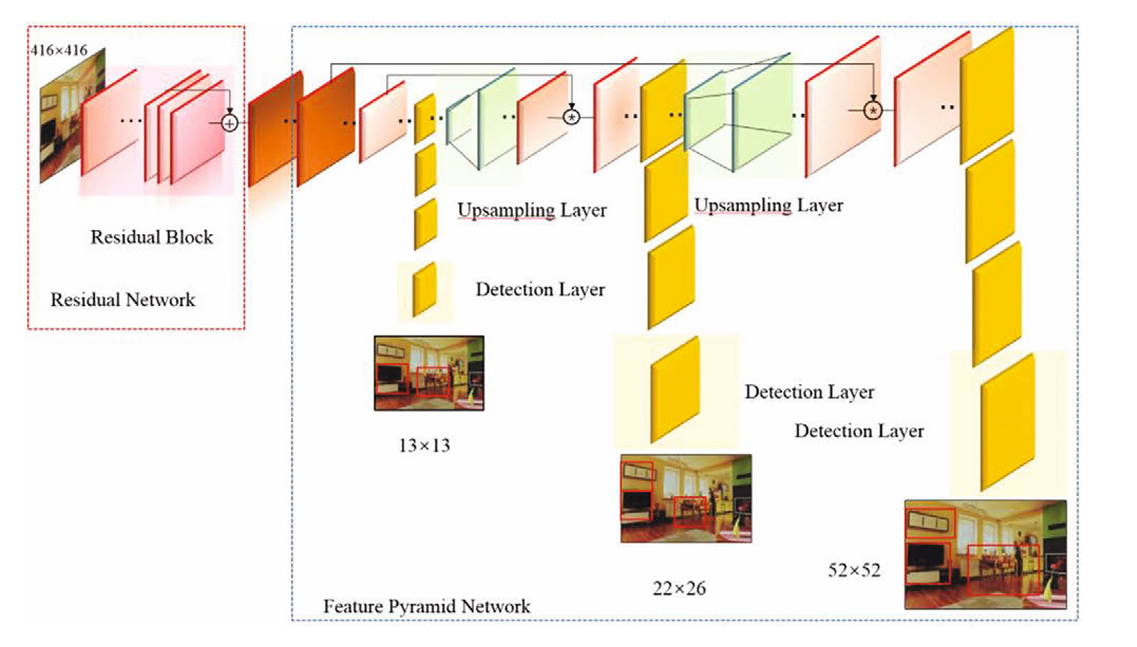
\includegraphics[width=\textwidth]{detection_heads.png}
	\end{center}
	\caption{The overall backbone and the three scale detection heads of YOLO-v3. This is taken from \cite{face_detection_yolo}}
	\label{fig:detection_head}
\end{figure*}

The detection head for the first scale then adds two more Convolutional blocks. For the second scale prediction, we take the output of the network just where the first detection head is attached and then upscale it by 2X. We then concatenate this feature map with a feature map a couple of blocks before. The idea is to use earlier feature maps along with upscaled current feature maps to make predictions on a higher resolution. This helps with detecting medium and small objects. The second detection head is then attached here which then adds two more CNN blocks to make predictions. The process is repeated to get predictions for the third scale. 

The Darknet 53 backbone trained on ImageNet is the modified with these new layers. The combined model is then trained on MS COCO object detection dataset. The results are shown in Figure \ref{fig:detector_comparison}. The loss function is explained in the YOLO-v3 and YOLO-v1 papers. We used the same loss function. 

\section{Evaluation}
In this section, we describe how we adapted the YOLO-v3 for our purposes. 

\subsection{Dataset}
We used a scaled down version of KITTI dataset. It contains only 1 class for cars. There are 3712 training images with single labelled car to multiple cars in an urban environment. The test set consists of 3769 images. The train set contains many images without any labelled cars. We remove them and end up with only 3177 images. We then divide into train and validation sets with 80/20 split (2541, 636 images). 

 \subsection{Data Augmentation}
 We used data augmentation strategies like random crop. color jitter (randomly change brightness, contrast, hue, staturation), affine transformation (change zoom level, translate left and right, rotate, and shear), horizontal flip, random blurring, colour channel shuffling, and grey scale. All these were applied with various probabilities. Finally the images are standardized (mean 0, std 1). These transforms are also applied to the bounding box labels. These data augmentation strategies reduce overfitting and make the model robust to colour variation due to weather and lightning, camera angles, artifacts and more.

 \subsection{Training Strategy}
We download the pretrained weights of YOLO-v3 for MS COCO. We then finetune the model using transfer learning. We first change the last layer in each scale to adapt the output for only 1 class instead of 80 in MS COCO. 

We then freeze all the layers except the last layer in each scale. This means that all layers contribute to forward pass but the gradients in backward pass are only calculated for the last layer in each scale. We used Adams optimizer with a weight decay of 1e-04. The YOLO loss function is a weighted sum of classification loss, no object loss, objectness score loss and bounding box coordinate loss. Their weights are initially set as (1, 10, 1, 10), respectively.

We trained on our train set for 20 epochs on a learning rate of 3e-05.  The loss went down but the rate of decrease stagnated at the end. 

We then unfreeze all the layers in each detection head. We then trained for 30 more epochs on a learning rate of 3e-05 and faced the same problem. 

We also observed that at this stage the model has perfect classification accuracy because there is only 1 class. The network has a bad no object score (predicting bounding boxes with high objectness score in grid cells with no objects) and it still performed badly in localizing the bounding boxes (quantified by IOU between ground truth and pred box). We therefore changed the weights of the loss to (1, 15, 10, 20). Namely, we increased the no object penalty by 1.5 times, we increase the objectness score penalty by 10 times, and we double the weight of bounding box coordinates loss. We then train for 10 more epochs.

Finally, we unfreeze two more CNN blocks before each detection head. This means that the CNN blocks before each head now also receive gradient and are updated. We decrease the learning rate to 1e-05 and train for further 60 more epochs. 

The above training procedure is not planned but reactive in nature as we trained and observed the model performance and tweaked parameters. 

\subsection{Discussion and Results}
We acheived a mAP of 51 percent on both the training set and validation set. We never used the validation set for any automated hyperparameter optimization. Therefore our test accuracy is likely to be around 51 percent mAP as well. 

Beyond the accuracy metric, we observed that our model has some trouble properly localizing some cars. We think this is due to many reasons.

First, we used the anchor boxes suitable for MS COCO. Our dataset has only rectangular objects. Using anchor boxes well suited for cars should improve mAP. 

Second, our training procedure should be optimized. Hyperparameter optimization in terms of learning rate schedules, how many layers to unfreeze, and loss weights can be done with more time and GPU compute at hand (which we did not have). Some sample predictions of the model on test set can be seen in Figure \ref{fig:pred_example_plot} and Figure \ref{fig:pred_example_plot2}. We observed that sometimes the model confused motorists, trains and trucks with cars. We think that this can be improved by including labels for those classes as well. Finally, we think that training on a larger, more diverse dataset with higher resolution images should improve car detection for practical applications.

\begin{figure}[t]
	\begin{center}
		%\fbox{\rule{0pt}{2in} \rule{0.9\linewidth}{0pt}}
		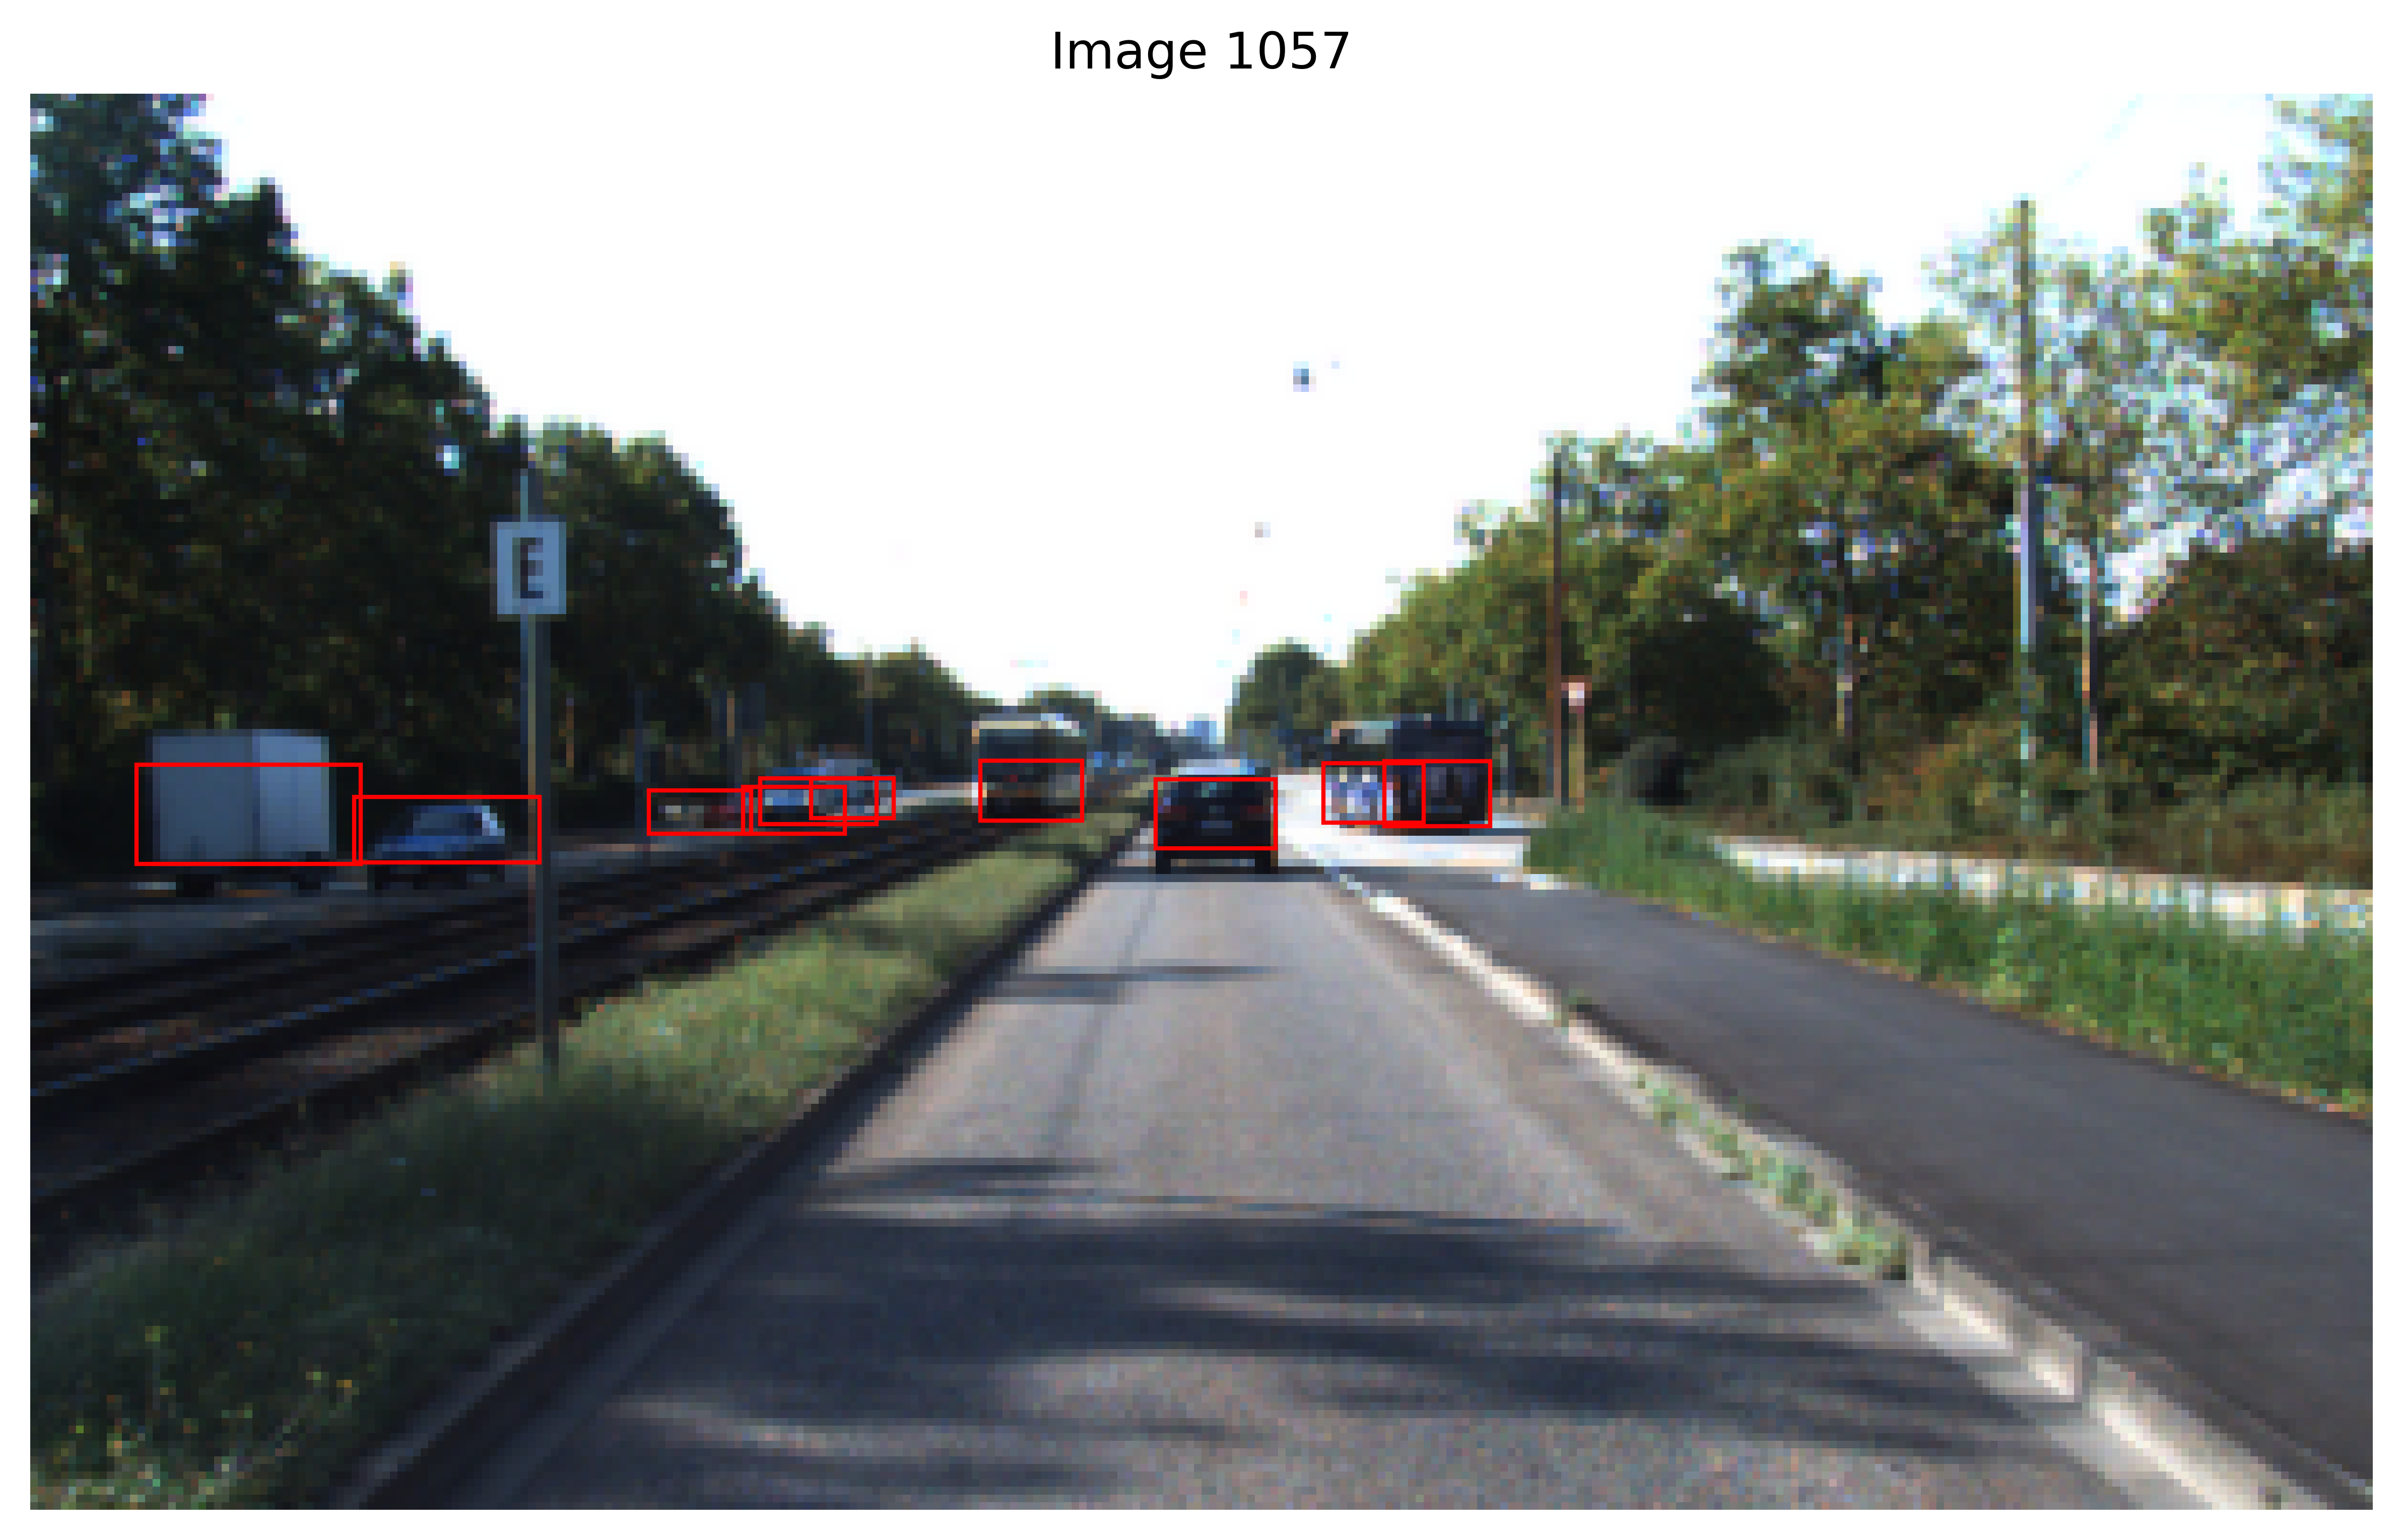
\includegraphics[width=1.0\linewidth]{figure1057.png}
	\end{center}
	\caption{Detections of the model developed in this project on a sample image from the test set.}
	\label{fig:pred_example_plot2}
\end{figure}


\begin{table}
	\begin{center}
		\begin{tabular}{|l|c|}
			\hline
			Set & mAP \\
			\hline\hline
			Train & 0.51 \\
			Validation & 0.51\\
			\hline
		\end{tabular}
	\end{center}
	\caption{Results. The mAP is calculated using PASCAL VOC 2007 metric using instructor provided code.}
	\label{tab:results}
\end{table}

\section{Conclusion and Future Work}
We adapted YOLO-v3 2D object detector to perform car detection on a scaled down version of KITTI dataset. We acheived a mAP of 51 percent. Hyperparameter optimization is required in terms of finetuning the pretrained model on our dataset. Clustering analysis can be done to find better anchor boxes. These measures should improve performance. In future, newer object detection frameworks based on Detection Transformer should be investigated. We learned about 2D object detection by doing this project and coded many things from scratch.
\section{Acknowledgments}
We adapted a Pytorch implementation of YOLO-v3 by \cite{yolov3pytorch2022}.

%-------------------------------------------------------------------------

{\small
\bibliographystyle{ieee_fullname}
\bibliography{literature}
}

\end{document}
